\begin{figure}[t]
\centering
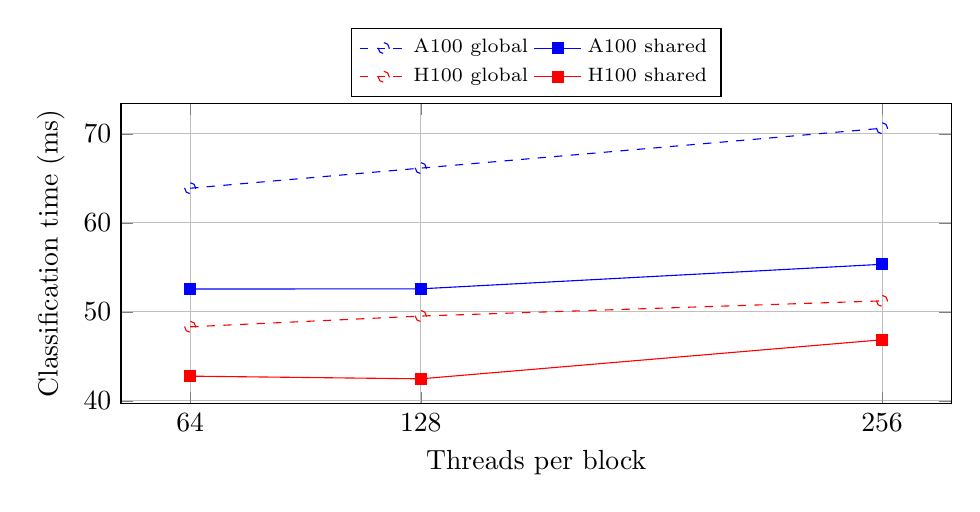
\begin{tikzpicture}
\begin{axis}[width=\columnwidth,height=5.4cm,xlabel={Threads per block},ylabel={Classification time (ms)},xtick={64,128,256},legend style={font=\scriptsize,at={(0.5,1.02)},anchor=south,legend columns=2},grid=major]
\addplot[blue,dashed,mark=o] coordinates {(64,63.889098) (128,66.14855) (256,70.62373533333333)};
\addlegendentry{A100 global}
\addplot[blue,solid,mark=square*] coordinates {(64,52.562508666666666) (128,52.589258666666666) (256,55.343317666666664)};
\addlegendentry{A100 shared}
\addplot[red,dashed,mark=o] coordinates {(64,48.321567333333334) (128,49.530923666666666) (256,51.233959)};
\addlegendentry{H100 global}
\addplot[red,solid,mark=square*] coordinates {(64,42.779333333333334) (128,42.47874233333333) (256,46.863927000000004)};
\addlegendentry{H100 shared}
\end{axis}\end{tikzpicture}
\caption{Large-dataset block-size experiment, three-run means from the paired sweeps. Hardware differs between A100 and H100.}\label{fig:gpu}
\end{figure}
